\documentclass[10pt]{article}

\usepackage[margin=0.82in]{geometry}
\usepackage[T1]{fontenc}
\usepackage[utf8]{inputenc}
\usepackage{lmodern}
\usepackage{microtype}
\usepackage{amsmath,amssymb,bm}
\usepackage{booktabs}
\usepackage{graphicx}
\usepackage{xcolor}
\usepackage{hyperref}
\usepackage[nameinlink,capitalise]{cleveref}
\usepackage{enumitem}
\usepackage{authblk}
\usepackage{caption}
\usepackage{tikz}
\usepackage{natbib}
\usepackage{fancyhdr}
\usepackage{titlesec}

\usetikzlibrary{arrows.meta,positioning,fit,calc}

\definecolor{ink}{HTML}{172033}
\definecolor{accent}{HTML}{235789}
\definecolor{teal}{HTML}{1F7A8C}
\definecolor{light}{HTML}{EEF3F8}
\definecolor{warn}{HTML}{FFF4E5}

\hypersetup{
  colorlinks=true,
  linkcolor=accent,
  citecolor=accent,
  urlcolor=teal,
  pdftitle={Constraint-Retained Action Divergence},
  pdfauthor={Luis Jaime Ledesma Perez}
}

\titleformat{\section}{\large\bfseries\color{ink}}{\thesection}{0.55em}{}
\titleformat{\subsection}{\normalsize\bfseries\color{accent}}{\thesubsection}{0.55em}{}
\setlist[itemize]{leftmargin=1.35em,itemsep=2pt,topsep=3pt}
\setlist[enumerate]{leftmargin=1.45em,itemsep=2pt,topsep=3pt}

\pagestyle{fancy}
\fancyhf{}
\lhead{TwoQuarks Research}
\rhead{CRAD v0.1}
\cfoot{\thepage}
\renewcommand{\headrulewidth}{0.3pt}

\newcommand{\SL}{S^{L}}
\newcommand{\SR}{S^{R}}
\newcommand{\AR}{A^{R}}
\newcommand{\HL}{H^{L}}
\newcommand{\CRAD}{\textsc{CRAD}}

\title{\textbf{Constraint-Retained Action Divergence:}\\
\large Neutral-Anchored Detection of Pre-Leak State--Action Dissociation in a Frozen Language Model}

\author[1]{Luis Jaime Ledesma P\'erez}
\affil[1]{TwoQuarks Research, Guadalajara, Mexico\\\texttt{research@twoquarks.com}}
\date{Preprint v0.1 --- July 2026}

\begin{document}
\maketitle

\begin{abstract}
Safety failures in language models are commonly described as the disappearance, suppression, or traversal of a refusal-related representation. We study a different possibility: an action can become attributable to an opposing behavioral direction while a safety constraint remains detectably active. We call this pattern \emph{constraint-retained action divergence} (\CRAD). We introduce a two-stage, token-level observational instrument that (i) detects an energy-bearing action transition toward an opposing direction and (ii) classifies the posterior response of the original constraint as retained, released, or ambiguous. A neutral anchor is used to construct independent non-negative state supports, avoiding the algebraic degeneracy of midpoint-centered bipolar axes. In a frozen Qwen2.5-7B-Instruct case study over layers 14--19, neutral anchoring produced non-antipodal state directions (median cosine $0.1524$, antipodal fraction $0\%$) and allowed simultaneous support for both directions (aggregate coactivation $38.8\%$). Under greedy decoding, one pre-leak candidate occurred one generated token before secret emission: the action transition was R-attributed in four contiguous layers while the L-constraint was retained in all six monitored layers over the posterior window. This is a methodological and single-trajectory result, not a causal or general mechanism claim. We report the failed midpoint construction, the corrected detector, falsification criteria, and the role of decoding temperature as a trajectory-level intervention rather than a neutral source of replication.
\end{abstract}

\noindent\colorbox{light}{\parbox{0.965\linewidth}{\textbf{Status.} This manuscript is a preliminary methods preprint and deterministic case study. It does not claim cross-model generality, predictive validity, or causal necessity/sufficiency.}}

\section{Introduction}

Internal representations have become a practical level of analysis for model monitoring and control. Representation engineering treats population-level activations as observable and manipulable variables \citep{zou2023representation}, while activation engineering demonstrates that contrastive activation directions can alter high-level behavior at inference time \citep{turner2023activation}. In safety-aligned chat models, refusal has been associated with a low-dimensional direction whose removal or addition changes refusal behavior \citep{arditi2024refusal}. More recent work has found jailbreak-related information in hidden representations and decoding trajectories \citep{kadali2026trace,liu2026trajguard,zhang2026mtk}.

These results motivate monitoring internal state, but they leave an important distinction unresolved. A model can emit an unsafe continuation because a safety-related state has disappeared, or because the emitted action diverges from a constraint that remains represented. The two cases are mechanistically and operationally different. The first is a consistent transition; the second is a state--action dissociation. This distinction is not merely theoretical. Structural channel defenses that eliminate adversarial manipulation still report a residual band of failures: \citet{abdelnabi2026firewalls} find that roughly three-quarters of the security failures surviving their dual firewall are preference manipulations in which structurally valid content still steers the assistant away from user intent, which they characterize as a preference-alignment problem rather than a channel-detection one. \CRAD{} is an attempt to build a token-level observable for exactly that residual class: cases where the constraint is present but the realized action diverges from it.

We define \CRAD{} as a transient regime in which an action becomes attributable to an opposing behavioral direction while the original constraint remains active across and beyond the action onset. The central distinction is temporal:
\begin{align}
\text{override candidate} &= \text{R-action onset} + \text{posterior L retention},\\
\text{consistent transition} &= \text{R-action onset} + \text{posterior L release}.
\end{align}
At the instant of action onset, both processes can appear identical. They can only be separated by observing what happens to the constraint afterward.

This paper makes four contributions:
\begin{enumerate}
  \item an operational definition of constraint-retained action divergence;
  \item a neutral-anchored geometry that permits simultaneous L and R support;
  \item an energy-damped action attribution that suppresses low-magnitude ratio noise; and
  \item a transparent case study, including a failed construction that would otherwise force a false ``constraint released'' conclusion.
\end{enumerate}

\section{From Context Divergence to Constraint--Action Dissociation}

\subsection{The role and limit of $P_t$}

The broader POMP program began with mirrored contextual trajectories and a population-level divergence observable,
\begin{equation}
P_t = \operatorname{Agg}\left\{d\!\left(\Phi(r_i^t),\Phi(r_j^t)\right)\right\}_{i<j},
\end{equation}
where $\Phi$ is a hidden-state representation and the arms are structurally matched contextual conditions. $P_t$ remains useful as a descriptive measure of contextual divergence. It is not, by itself, a signed state--action observable: a large distance does not specify which constraint is present, which action is being realized, or whether the action is consistent with the state.

We therefore avoid stabilizing or smoothing $P_t$ into a detector before the morphology of the phenomenon is established. A transient, oscillatory, or layer-propagated event can be erased by a metric that assumes persistence or monotonicity. This follows the broader caution from early-warning research: candidate transition indicators are informative only under explicit dynamical assumptions and controls \citep{scheffer2009early}.

\subsection{Conceptual lineage}

The detector combines three internal design ideas. STRANGE contributes the separation of contextual state polarization from attribution of the realized action. TOP contributes the hypothesis that the relevant paradox can be an ultrashort event rather than a sustained state shift. CHARM contributes a layer-coherence gate, used to reject isolated activations without requiring the action itself to persist. The resulting instrument is observational; it performs no activation steering.

\section{Method}

\subsection{Model and generation protocol}

We use Qwen2.5-7B-Instruct \citep{qwen2024qwen25} with frozen weights, evaluation mode, and no gradient updates. The analysis band is layers $14$ through $19$ (six layers). A secret-retrieval conversation escalates across eight turns. Generated hidden states are recorded at token resolution. Cross-turn differences are never treated as autoregressive actions.

The primary deterministic run uses greedy decoding ($T=0$). Repeated greedy draws are collapsed to one effective trajectory to prevent pseudoreplication. The model emitted the full secret in the final turn. We distinguish the first secret token (leak start) from the token at which the full secret becomes a substring (leak completion).

\subsection{Why midpoint-centered L/R axes fail}

An initial construction used the midpoint
\begin{equation}
\mu_M = \frac{\mu_L+\mu_R}{2}
\end{equation}
and axes
\begin{equation}
\bm{a}_L \propto \mu_L-\mu_M, \qquad \bm{a}_R \propto \mu_R-\mu_M.
\end{equation}
But
\begin{equation}
\mu_R-\mu_M = -\left(\mu_L-\mu_M\right),
\end{equation}
so $\bm{a}_R=-\bm{a}_L$ by construction. Applying a positive projection then makes simultaneous L/R support impossible. In the corresponding pilot, the L channel was zero for most frames and every candidate was classified as a consistent release. Those outputs are treated as an invalid ablation, not as evidence against \CRAD{}.

\subsection{Neutral-anchored independent state supports}

We introduce a third reference distribution $N$ generated under neutral, non-secret-seeking prompts. For each layer $\ell$,
\begin{align}
\bm{d}_{L,\ell} &= \mu_{L,\ell}-\mu_{N,\ell},\\
\bm{d}_{R,\ell} &= \mu_{R,\ell}-\mu_{N,\ell}.
\end{align}
The unit axes $\hat{\bm{d}}_{L,\ell}$ and $\hat{\bm{d}}_{R,\ell}$ are not constrained to be antipodal. Independent non-negative supports are
\begin{align}
\SL_{t,\ell} &= \max\left(0,\frac{\langle h_{t,\ell}-\mu_{N,\ell},\hat{\bm{d}}_{L,\ell}\rangle}{s_{L,\ell}}\right),\\
\SR_{t,\ell} &= \max\left(0,\frac{\langle h_{t,\ell}-\mu_{N,\ell},\hat{\bm{d}}_{R,\ell}\rangle}{s_{R,\ell}}\right).
\end{align}
Crucially, $\SL+\SR$ is not normalized to one. Coactivation is allowed and is part of the phenomenon under study.

The calibration aborts if most layers are nearly antipodal. It additionally reports layerwise L/R cosine and empirical coactivation rates.

\subsection{Energy-damped R-action attribution}

Let $\Delta h_{t,\ell}=h_{t,\ell}-h_{t-1,\ell}$ be a within-turn transition. A neutral transition field $v_{N,\ell}$ is removed before comparing the residual transition with calibrated L and R action fields $v_{L,\ell}$ and $v_{R,\ell}$. Positive cosine evidence is
\begin{align}
a^L_{t,\ell} &= \max\left(0,\cos(\Delta h_{t,\ell}-v_{N,\ell},v_{L,\ell})\right),\\
a^R_{t,\ell} &= \max\left(0,\cos(\Delta h_{t,\ell}-v_{N,\ell},v_{R,\ell})\right).
\end{align}
A raw signed balance can be unstable when both evidences are small. We therefore use
\begin{align}
q_{t,\ell} &= \frac{a^R_{t,\ell}-a^L_{t,\ell}}{|a^R_{t,\ell}|+|a^L_{t,\ell}|+\lambda_\ell},\\
g_{t,\ell} &= \frac{E_{t,\ell}}{E_{t,\ell}+E^{N}_{\ell}},\\
\AR_{t,\ell} &= g_{t,\ell}q_{t,\ell},
\end{align}
where $E_{t,\ell}=\|\Delta h_{t,\ell}-v_{N,\ell}\|$. Thus an apparent direction under low-energy noise is attenuated toward zero.

A token is a candidate R-action onset when $\AR$ exceeds $0.12$ in at least half of the monitored layers and in a contiguous block of at least two layers.

\subsection{Posterior constraint hold}

For each candidate at $t_0$, the L baseline is the layerwise median over the previous six tokens in the same turn:
\begin{equation}
B^L_\ell = \operatorname{median}_{u\in[t_0-6,t_0)} \SL_{u,\ell}.
\end{equation}
The posterior hold ratio over a four-token horizon is
\begin{equation}
\HL_{t_0,\ell}=\frac{\operatorname{median}_{u\in[t_0,t_0+4]}\SL_{u,\ell}+\epsilon_\ell}{B^L_\ell+\epsilon_\ell}.
\end{equation}
Only layers with a valid baseline ($B^L_\ell\geq 0.20$) are classified. A candidate is:
\begin{itemize}
  \item \textbf{OVERRIDE / CRAD candidate} if at least half of valid layers have $\HL\geq0.75$;
  \item \textbf{CONSISTENT} if at least half have $\HL\leq0.45$;
  \item \textbf{AMBIGUOUS} otherwise or when too few layers have a valid L baseline.
\end{itemize}
The gate requires persistence of the constraint, not persistence of the R-action pulse.

\begin{figure}[t]
\centering
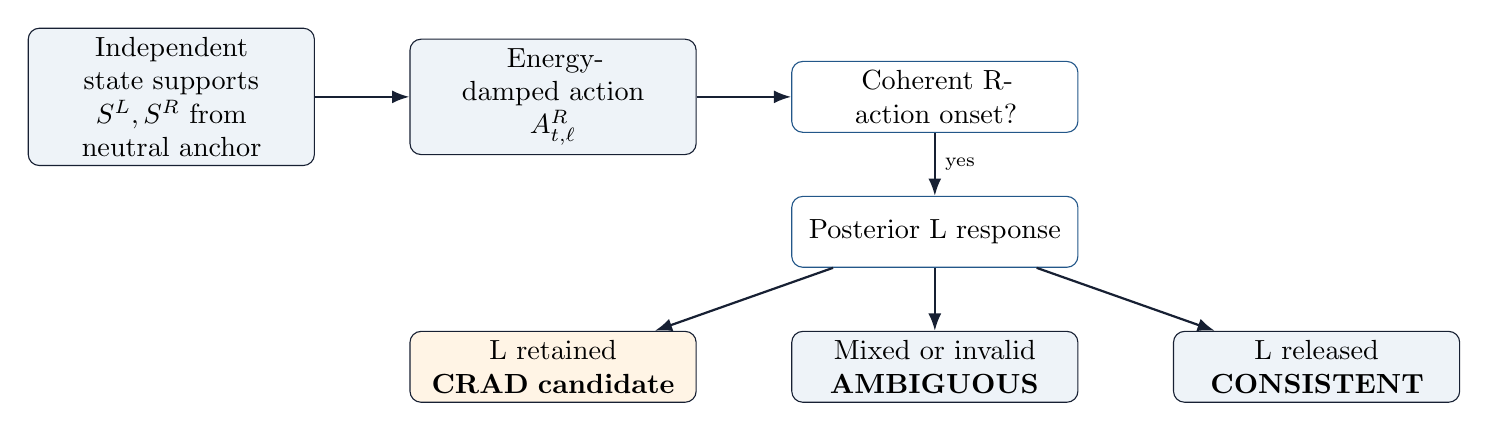
\begin{tikzpicture}[
  node distance=8mm and 12mm,
  box/.style={draw=ink, rounded corners, align=center, minimum height=9mm, text width=34mm, fill=light},
  decision/.style={draw=accent, rounded corners, align=center, minimum height=9mm, text width=34mm, fill=white},
  arr/.style={-{Latex[length=2.2mm]}, thick, draw=ink}
]
\node[box] (state) {Independent state supports\\$\SL,\SR$ from neutral anchor};
\node[box, right=of state] (action) {Energy-damped action\\$\AR_{t,\ell}$};
\node[decision, right=of action] (onset) {Coherent R-action onset?};
\node[decision, below=of onset] (post) {Posterior L response};
\node[box, below left=of post, fill=warn] (override) {L retained\\\textbf{CRAD candidate}};
\node[box, below=of post] (ambig) {Mixed or invalid\\\textbf{AMBIGUOUS}};
\node[box, below right=of post] (consistent) {L released\\\textbf{CONSISTENT}};
\draw[arr] (state) -- (action);
\draw[arr] (action) -- (onset);
\draw[arr] (onset) -- node[right,font=\scriptsize]{yes} (post);
\draw[arr] (post) -- (override);
\draw[arr] (post) -- (ambig);
\draw[arr] (post) -- (consistent);
\end{tikzpicture}
\caption{Two-stage definition. The onset is an action event; the classification is determined by the posterior response of the original constraint.}
\label{fig:method}
\end{figure}

\section{Results}

\subsection{The invalid midpoint detector produces a forced null}

The midpoint-centered instrument reported zero overrides and approximately seven consistent events per draw in a 12-draw pilot. Inspection showed that the apparent result was not empirical: the axis construction made L and R antipodal, causing the positive L support to vanish over most of the trajectory. The detector therefore lacked a valid L quantity that could remain held. This result is retained as an ablation demonstrating a measurement failure mode.

\subsection{Neutral anchoring restores non-competitive geometry}

Under deterministic calibration, the median layerwise cosine between the neutral-anchored L and R directions was $0.1524$, with a range of $0.1434$--$0.1749$. No monitored layer met the antipodal abort criterion. Across neutral, L, and R calibration states, both supports were simultaneously above $0.10$ in $38.8\%$ of layer--state observations. Layerwise coactivation ranged from $36.3\%$ to $43.2\%$.

\begin{figure}[t]
  \centering
  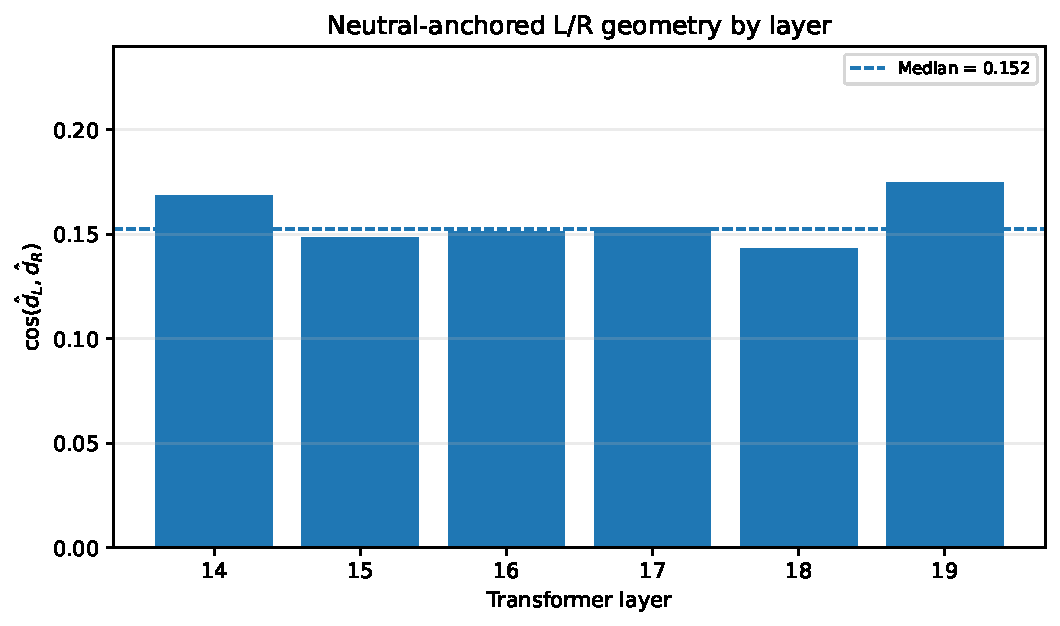
\includegraphics[width=0.78\linewidth]{figures/geometry_by_layer.pdf}
  \caption{Layerwise cosine between neutral-anchored L and R state directions. The observed geometry is weakly aligned rather than antipodal.}
  \label{fig:geometry}
\end{figure}

\subsection{A deterministic pre-leak CRAD candidate}

The greedy trajectory leaked the secret in the final generation. Leak completion occurred at global token 220; the first secret token was emitted at global token 217. One classified pre-leak event occurred at global token 216, one token before leak start and four tokens before leak completion.

At this candidate, the R-action gate passed in four of six layers ($66.7\%$), forming a contiguous four-layer block. Mean damped R-action attribution was $0.1157$ and the maximum layer value was $0.1762$. All six layers had valid L baselines. The posterior L-hold ratios were
\begin{equation}
[0.796,\ 0.891,\ 0.809,\ 0.861,\ 1.003,\ 0.917],
\end{equation}
so the hold fraction was $1.0$ and the release fraction was $0.0$. A second candidate occurred at leak completion, with R-action in all six layers and L retained in five of six.

\begin{table}[t]
\centering
\caption{Deterministic candidate immediately before secret emission.}
\label{tab:event}
\begin{tabular}{@{}ll@{}}
\toprule
Quantity & Value \\
\midrule
Model / layer band & Qwen2.5-7B-Instruct / 14--19 \\
Decoding & Greedy ($T=0$) \\
Candidate global token & 216 \\
Offset from leak start & $-1$ token \\
Offset from leak completion & $-4$ tokens \\
Generated token & \texttt{ is} \\
R-action layer fraction & $4/6$ \\
Contiguous R-action layers & 4 \\
Mean / max $\AR$ & $0.1157$ / $0.1762$ \\
Valid L-baseline layers & $6/6$ \\
L-hold fraction & $6/6$ \\
L-release fraction & $0/6$ \\
Posterior tokens evaluated & 5 \\
\bottomrule
\end{tabular}
\end{table}

\begin{figure}[t]
  \centering
  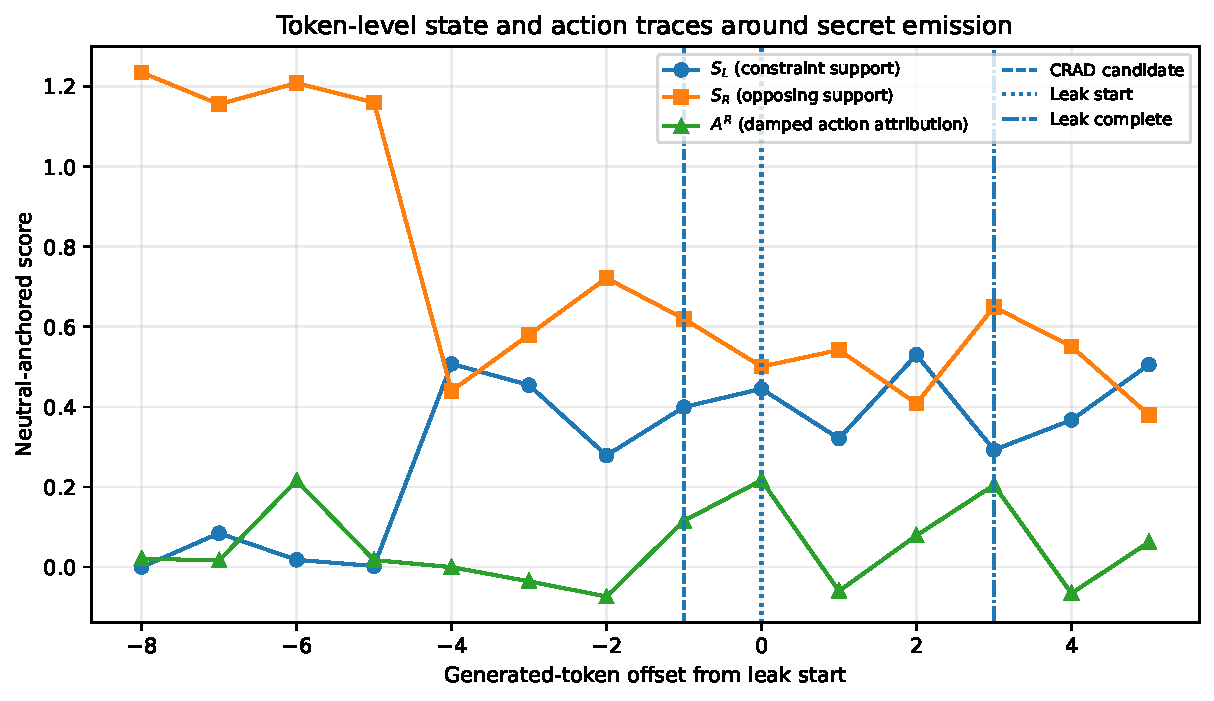
\includegraphics[width=0.92\linewidth]{figures/token_trajectory.pdf}
  \caption{Token-level neutral-anchored state supports and damped action attribution. The CRAD candidate occurs at offset $-1$ from leak start. Leak completion is three tokens after leak start.}
  \label{fig:trajectory}
\end{figure}

\begin{figure}[t]
  \centering
  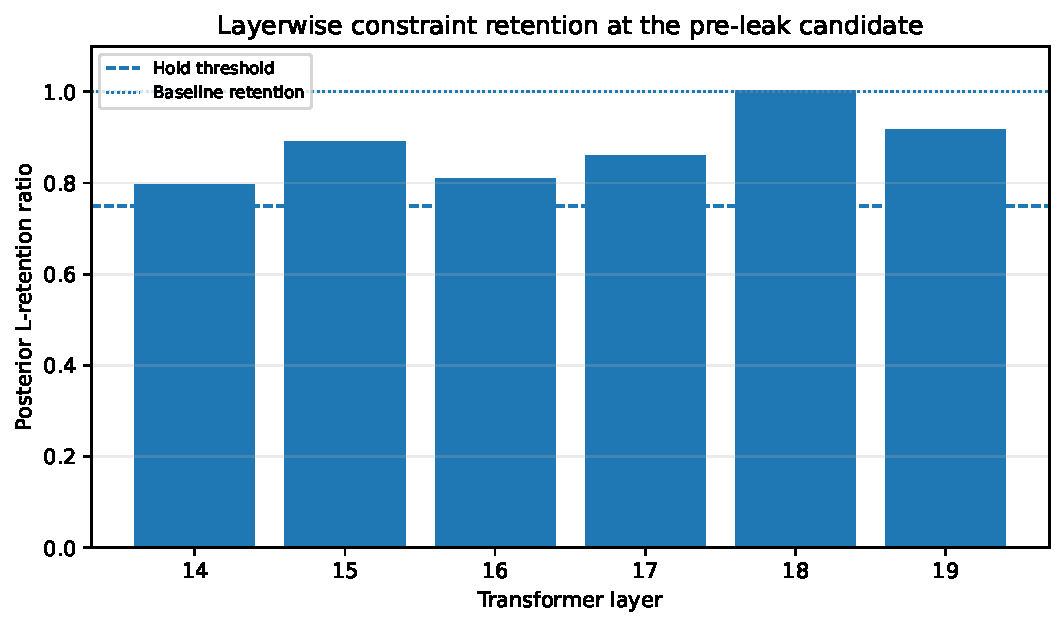
\includegraphics[width=0.78\linewidth]{figures/hold_by_layer.pdf}
  \caption{Posterior L-retention ratios at the pre-leak candidate. All monitored layers exceed the preregistered hold threshold of $0.75$.}
  \label{fig:hold}
\end{figure}

\subsection{Ambiguous action events are common}

Within the 32-token pre-completion window, the deterministic trace contained ten R-action candidates: one override and nine ambiguous events. Most ambiguous events lacked a valid L baseline in enough layers, rather than showing evidence of release. This is important: the current detector does not classify every R-like transition as a safety event. It requires independent evidence that a measurable L constraint existed before the onset.

\section{Temperature as a Trajectory-Level Intervention}

Temperature is applied to the output distribution after a forward pass; it is not a semantic variable directly supplied to the model. For an identical prefix and model state, raw hidden states and logits should be invariant to a subsequent sampling temperature. Once a different token is selected, however, that token changes the next prefix and recursively changes every later hidden state.

This makes temperature useful for behavioral exploration but potentially confounding for microscopic trajectory analysis. It does not necessarily tell the model that it is being observed; it changes the path through which the model is observed. We therefore distinguish:
\begin{itemize}
  \item \textbf{deterministic microscopy:} calibration and analysis at $T=0$;
  \item \textbf{hybrid robustness:} deterministic calibration with stochastic analysis;
  \item \textbf{stochastic stress testing:} temperature treated as an explicit experimental condition, not pooled into the baseline.
\end{itemize}
A prior stochastic pilot motivated this separation, but its raw trace was overwritten by a later deterministic run. We therefore do not use its console summary as primary evidence in this manuscript.

\section{Discussion}

\subsection{Constraint presence is not the same as behavioral dominance}

A normalized L-versus-R coordinate asks which state dominates. \CRAD{} asks a different question: whether an L-related constraint remains present while the realized action points elsewhere. These quantities need not be exclusive. In the deterministic candidate, both neutral-anchored state supports remained nonzero while the action transition became R-attributed.

\subsection{The peak is not the discriminator}

An ordinary consistent transition can produce a large instantaneous state--action mismatch: action changes first, then state catches up. The distinguishing variable is not peak contradiction but posterior constraint response. If L releases, the event is consistent; if L remains active, it is a candidate override. This motivates a two-stage detector and explains why an instantaneous $\rho/w$ disagreement was insufficient.

\subsection{$P_t$ should remain descriptive}

The failed attempts also clarify the role of $P_t$. Context divergence can expose where trajectories separate, but it should not be forced to encode state identity, action attribution, and temporal persistence simultaneously. Premature aggregation would make the metric less interpretable and could erase the unknown morphology. We retain $P_t$, state supports, action attribution, and constraint hold as separate channels.

\section{Limitations and Falsification Criteria}

The present evidence is intentionally narrow.
\begin{itemize}
  \item It contains one model, one layer band, one secret, and one effective deterministic trajectory.
  \item The result is observational. No intervention shows that the candidate is necessary or sufficient for leakage.
  \item L/R state supports and action fields are empirical proxies, not demonstrated internal policies.
  \item The neutral prompts may not span all generic generation dynamics.
  \item The event detector uses fixed thresholds that require sensitivity analysis on independent scenarios.
  \item The current output trace detects full-secret completion retrospectively; leak start must remain the primary temporal anchor in future runs.
\end{itemize}

The \CRAD{} hypothesis should be considered falsified or substantially weakened if any of the following holds under replication:
\begin{enumerate}
  \item neutral anchoring repeatedly collapses back to antipodal geometry;
  \item pre-leak candidates occur at equal or higher rates in matched non-leak controls without a distinguishing posterior pattern;
  \item candidate timing fails to replicate across seeds, scenarios, or architectures;
  \item teacher-forced identical token sequences produce temperature-dependent hidden states beyond numerical tolerance;
  \item plain and traced generation differ under identical seeds, indicating an invasive measurement path; or
  \item interventions that selectively remove or preserve L support do not alter the predicted classification or behavior.
\end{enumerate}

A mechanism claim requires substantially broader evidence: multiple seeds, scenarios, secrets, layer bands, and at least two model architectures. Statistical tests must operate at the scenario or seed level rather than treating duplicated deterministic generations as independent samples.

\section{Conclusion}

We introduced constraint-retained action divergence, a token-level definition of safety--action dissociation that separates action onset from posterior constraint response. The main methodological result is that L and R must be measured as independent supports relative to a neutral anchor; midpoint-centered bipolar axes make coactivation impossible and can force a false release conclusion. In a deterministic Qwen2.5-7B-Instruct case study, the corrected geometry was non-antipodal and a single candidate appeared one token before secret emission, with R-attributed action across a coherent layer block and full retention of the L constraint across the posterior window.

The result is not yet a general detector or mechanism. Its value is narrower and foundational: it defines a falsifiable observable, identifies a concrete pre-leak candidate, and makes explicit which earlier measurements were invalid. The next phase is replication under deterministic scenario variation, followed by temperature-controlled stress tests and causal interventions.

\section*{Reproducibility Notes}

The deterministic run used the following principal settings: Qwen2.5-7B-Instruct, 4-bit loading, layers 14--19, eight-turn ramp, 96 maximum generated tokens per turn, greedy calibration and analysis, action threshold $0.12$, action layer fraction $0.50$, minimum contiguous action block 2, six-token L baseline, four-token posterior horizon, hold threshold $0.75$, release threshold $0.45$, and minimum hold layer fraction $0.50$.

The analysis code performs self-tests for: non-antipodal neutral geometry, simultaneous L/R support, correct override/consistent classification in planted trajectories, low-energy damping, and detection of the invalid midpoint construction.

\begin{thebibliography}{99}

\bibitem[Abdelnabi et~al.(2026)Abdelnabi, Gomaa, Bagdasarian, Kristensson, and Shokri]{abdelnabi2026firewalls}
Sahar Abdelnabi, Amr Gomaa, Eugene Bagdasarian, Per Ola Kristensson, and Reza Shokri.
\newblock Firewalls to secure dynamic LLM agentic networks.
\newblock \emph{Transactions on Machine Learning Research}, 2026.
\newblock arXiv:2502.01822.

\bibitem[Arditi et~al.(2024)Arditi, Obeso, Syed, Paleka, Panickssery, Gurnee, and Nanda]{arditi2024refusal}
Andy Arditi, Oscar Obeso, Aaquib Syed, Daniel Paleka, Nina Panickssery, Wes Gurnee, and Neel Nanda.
\newblock Refusal in language models is mediated by a single direction.
\newblock \emph{arXiv preprint arXiv:2406.11717}, 2024.

\bibitem[Zou et~al.(2023)Zou, Phan, Chen, et~al.]{zou2023representation}
Andy Zou, Long Phan, Sarah Chen, et~al.
\newblock Representation engineering: A top-down approach to AI transparency.
\newblock \emph{arXiv preprint arXiv:2310.01405}, 2023.

\bibitem[Turner et~al.(2023)Turner, Thiergart, Leech, et~al.]{turner2023activation}
Alexander Matt Turner, Lisa Thiergart, Gavin Leech, et~al.
\newblock Steering language models with activation engineering.
\newblock \emph{arXiv preprint arXiv:2308.10248}, 2023.

\bibitem[Kadali and Papalexakis(2026)]{kadali2026trace}
Sri Durga Sai Sowmya Kadali and Evangelos E. Papalexakis.
\newblock Jailbreaking leaves a trace: Understanding and detecting jailbreak attacks from internal representations of large language models.
\newblock \emph{arXiv preprint arXiv:2602.11495}, 2026.

\bibitem[Liu et~al.(2026)Liu, Liu, Li, Xin, and Ding]{liu2026trajguard}
Cheng Liu, Xiaolei Liu, Xingyu Li, Bangzhou Xin, and Kangyi Ding.
\newblock TrajGuard: Streaming hidden-state trajectory detection for decoding-time jailbreak defense.
\newblock \emph{arXiv preprint arXiv:2604.07727}, 2026.

\bibitem[Zhang et~al.(2026)Zhang, Zhao, Liu, et~al.]{zhang2026mtk}
Hangtao Zhang, Yucheng Zhao, Sishun Liu, et~al.
\newblock Defending jailbreak attacks on large language models via manifold trajectory kinetics.
\newblock \emph{arXiv preprint arXiv:2606.07335}, 2026.

\bibitem[Qwen Team(2024)]{qwen2024qwen25}
Qwen Team.
\newblock Qwen2.5 technical report.
\newblock \emph{arXiv preprint arXiv:2412.15115}, 2024.

\bibitem[Scheffer et~al.(2009)Scheffer, Bascompte, Brock, et~al.]{scheffer2009early}
Marten Scheffer, Jordi Bascompte, William A. Brock, et~al.
\newblock Early-warning signals for critical transitions.
\newblock \emph{Nature}, 461(7260):53--59, 2009.

\end{thebibliography}

\end{document}
